\chapter{Implementation of the method for unidirectional waves}
The JONSWAP spectrum is defined as
\begin{subequations}
\begin{equation}
    S_{\eta \eta}(f) = \alpha H_s^2 f_p^4 f^{-5} \gamma^\beta \exp{\left[-\frac{5}{4}\left(\frac{f_p}{f}\right)^4\right]}
    \label{eq:JONSWAPSpec}
\end{equation} 
\begin{equation}
    \alpha \approx \frac{0.0624}{0.230+0.0336\gamma-\frac{0.185}{1.9+\gamma}} ,\quad \beta = \exp{\left[ -\frac{(f-f_p)^2}{2\sigma^2f_p^2} \right]}, \quad
    \sigma =
    \begin{cases}
    0.07, \quad \text{for }f\leq f_p \\
    0.09, \quad \text{for }f> f_p
    \end{cases}
    \label{eq:JONSWAPparam}
\end{equation}
\end{subequations}
where \cref{eq:JONSWAPSpec} defines the power spectrum and \cref{eq:JONSWAPparam} defines the suggested scalar parameters given in the slides. Here, $H_s$ is the significant wave height, $f_p$ is the frequency corresponding to the peak period (i.e. $f_p=1/T_p$), $f$ is the frequency of interest, $\gamma$ is the so-called peak enchancement factor and $\alpha$, $\beta$, $\sigma$ are scalar parameters describing the shape of the JONSWAP spectrum.

\begin{figure}[htbp]
    \centering
    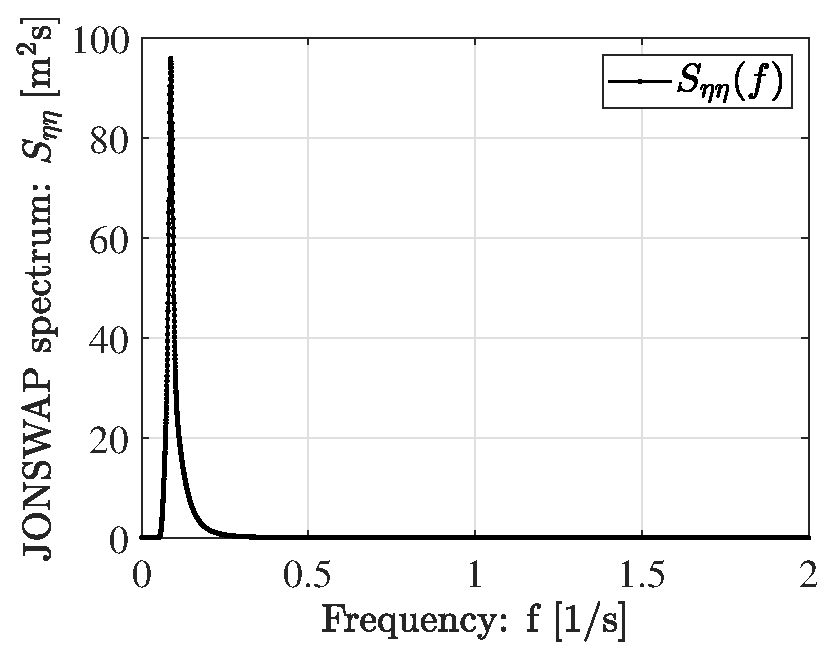
\includegraphics[width=0.5\textwidth]{Figures/Plots/JONSWAPres.eps}
    \caption{Caption}
    \label{fig:my_label}
\end{figure}

\begin{figure}[htbp]
    \centering
    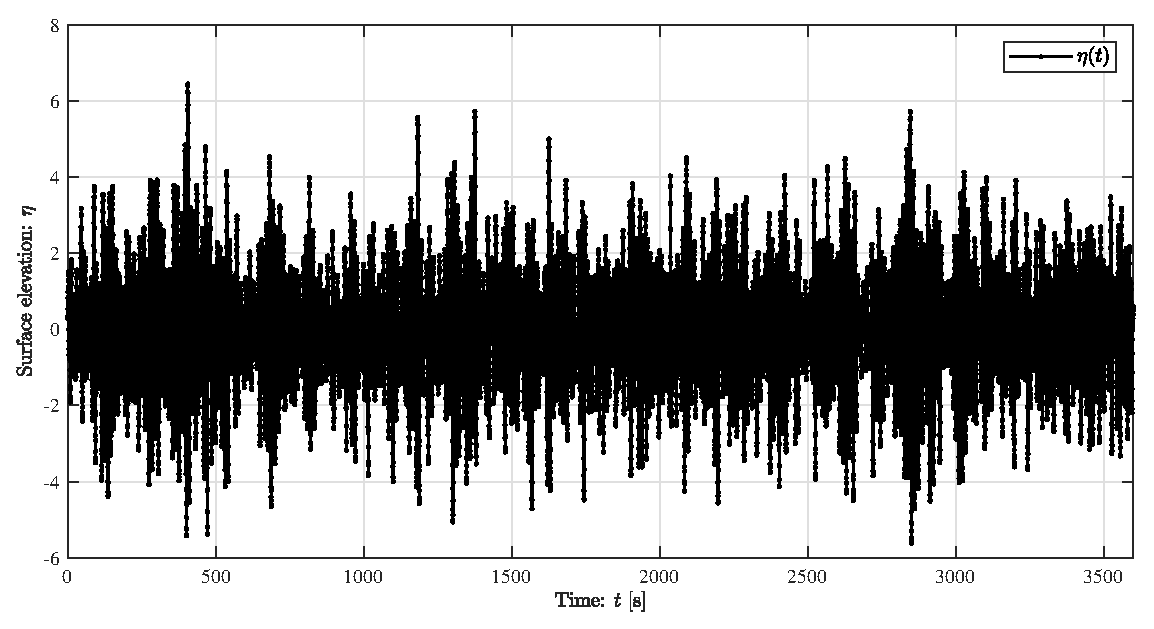
\includegraphics[width=0.9\textwidth]{Figures/Plots/SurfaceElevation.eps}
    \caption{Caption}
    \label{fig:my_label}
\end{figure}